%%%%%%%%%%%%%%%%%%%%%%%%%%%%%%%%%%%%%%%%%%%%%%%%%%%%%%%%%%%%%%%%%%%%%%%%%%%%
\begin{frame}[fragile]\frametitle{}

\begin{center}
{\Large Medical NER with spaCy}

{\tiny (Ref: Med7 — an information extraction model for clinical natural language processing - Kormilitzin)}
\end{center}


\end{frame}


%%%%%%%%%%%%%%%%%%%%%%%%%%%%%%%%%%%%%%%%%%%%%%%%%%%%%%%%%%%%%%%%%%%%%%%%%%%%%%%%%%
\begin{frame}[fragile]\frametitle{Background}
  \begin{itemize}
  \item Majority of patients' medical records are now being collected electronically
	\item A true asset for research, personalised approach to treatments
	\item However, the majority of patients’ information is contained in a free-text form as summarised by clinicians, nurses and care givers
	\item NLP/NER can extract meaningful information from unstructured medical records
  \end{itemize}
	
\end{frame}

%%%%%%%%%%%%%%%%%%%%%%%%%%%%%%%%%%%%%%%%%%%%%%%%%%%%%%%%%%%%%%%%%%%%%%%%%%%%%%%%%%
\begin{frame}[fragile]\frametitle{Med7}
  \begin{itemize}
  \item Dedicated named-entity recognition model Med7 for identification of 7 medication-related concepts, dosage, drug names, duration, form, frequency, route of administration and strength
	\item Trained on MIMIC-III,openly available dataset by MIT
	\item Comprises EHR from over 60,000 intensive care unit admissions, structured and unstructured medical records
	\item Open source and freely available python package for spaCy
	\item Models with pre-trained spaCy weights
  \end{itemize}
	

\begin{center}
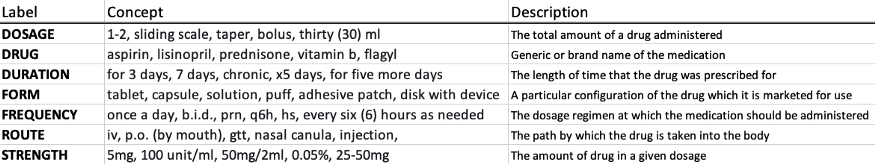
\includegraphics[width=0.8\linewidth,keepaspectratio]{spacy1}
\end{center}

	
\end{frame}


%%%%%%%%%%%%%%%%%%%%%%%%%%%%%%%%%%%%%%%%%%%%%%%%%%%%%%%%%%
\begin{frame}[fragile]\frametitle{Installation}


\begin{lstlisting}
(base) conda create -n med7 python=3.7
(base) conda activate med7
(med7) pip install -U spacy
(med) pip install https://med7.s3.eu-west-2.amazonaws.com/en_core_med7_lg.tar.gz

\end{lstlisting}


\end{frame}

%%%%%%%%%%%%%%%%%%%%%%%%%%%%%%%%%%%%%%%%%%%%%%%%%%%%%%%%%%
\begin{frame}[fragile]\frametitle{Usage}


\begin{lstlisting}
import spacy

med7 = spacy.load("en_core_med7_lg")

# create distinct colours for labels
col_dict = {}
seven_colours = ['#e6194B', '#3cb44b', '#ffe119', '#ffd8b1', '#f58231', '#f032e6', '#42d4f4']
for label, colour in zip(med7.pipe_labels['ner'], seven_colours):
    col_dict[label] = colour

options = {'ents': med7.pipe_labels['ner'], 'colors':col_dict}

text = 'A patient was prescribed Magnesium hydroxide 400mg/5ml suspension PO of total 30ml bid for the next 5 days.'
doc = med7(text)

spacy.displacy.render(doc, style='ent', jupyter=True, options=options)

[(ent.text, ent.label_) for ent in doc.ents]
\end{lstlisting}


\end{frame}

%%%%%%%%%%%%%%%%%%%%%%%%%%%%%%%%%%%%%%%%%%%%%%%%%%%%%%%%%%
\begin{frame}[fragile]\frametitle{Output}


\begin{lstlisting}
[('Magnesium hydroxide', 'DRUG'),
 ('400mg/5ml', 'STRENGTH'),
 ('suspension', 'FORM'),
 ('PO', 'ROUTE'),
 ('30ml', 'DOSAGE'),
 ('bid', 'FREQUENCY'),
 ('for the next 5 days', 'DURATION')]
\end{lstlisting}

also, it is possible to display the identified concepts:

\begin{center}
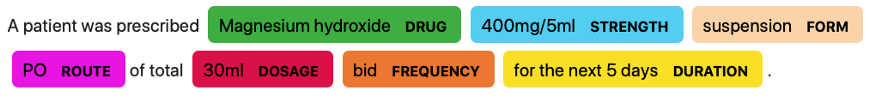
\includegraphics[width=0.8\linewidth,keepaspectratio]{spacy2}
\end{center}

\end{frame}